\documentclass{beamer}
\usepackage[utf8]{inputenc}
\usepackage{graphicx,url}
\usepackage{lmodern}
\usepackage{bm}
\usepackage{subcaption}
\usepackage{multicol}
\usepackage{makecell}
\usepackage{epstopdf}
\usepackage{graphicx}	
\usepackage[all]{xy}
\usepackage{amsmath}
\usepackage{mathrsfs}
\usepackage{epstopdf}
\usepackage{multirow}
\usepackage{amssymb}
\usepackage{mathtools}
\usepackage{animate}

\newcommand{\pag}[1] {\begin{frame}#1\end{frame}}
\DeclarePairedDelimiter\abs{\lvert}{\rvert}%
\newcommand{\norm}[1]{\left\lVert#1\right\rVert}
\newcommand{\tbf}[1]{\textbf{#1}}
\newcommand{\vect}[1]{\hat{\mathbf{#1}}}
\newcommand{\la}[1]{\mathrm{#1}}
\newcommand{\vc}[1]{\mathbf{#1}}
\newcommand{\vch}[1]{\hat{\mathbf{#1}}}
\usetheme[secheader]{Madrid}

\title{Constelações PAM e QAM}

\author[Silva]{\textbf{Higo Thaian Pereira da Silva \vspace{0.3cm} \\ Orientador: Prof. Dr. Marcelo Sampaio de Alencar
\vspace{0.3cm} \\ Coorientador: Prof. Dr. Wamberto José Lira de Queiroz} \vspace{0.3cm} \\ Universidade Federal de Campina Grande
(UFCG)}

\date[UFCG 2020]{UFCG, 3 de Dezembro, 2020}

\titlegraphic{\vspace*{-1.5cm}~
\includegraphics[scale=0.4]{UfcgBrasao.png}\hspace*{8cm}~%
   
\includegraphics[width=2cm]{IecomLogo.png}
}



\begin{document}

\frame{\titlepage}

\begin{frame}
  \frametitle{Roteiro}
  \tableofcontents
  % You might wish to add the option [pausesections]
\end{frame}

\section{Análise no Espaço de Sinais e Constelação}
\subsection{Representação Vetorial de Sinais}
\pag{
	\frametitle{Representação Vetorial de Sinais}
	\begin{itemize}
		\item 	Em um \textbf{sistema de comunicação digital}, a cada $T$ segundos são transmitidos $k$ bits de informação, \textbf{conformando uma taxa de transmissão de bit} de $R = k / T$ bits/s;
		\item 	É possível definir um total de $M = 2^{k}$ sequências distintas de $k$ bits, compondo um conjunto de {mensagens binárias} $\mathcal{M} = \{m_{1}, \cdots, m_{M}\}$;
		\item   Em um dado \textbf{intervalo de sinalização} $T$, uma mensagem binária $m_{i}$ é mapeada em um sinal analógico $s_{i}(t) \in \mathcal{S} = \{s_1(t),\cdots,s_{M}(t)\}$ que é transmitida por um canal;
		\begin{block}{Energia do sinal $s_{i}(t)$}
			\begin{equation}
				E_{s_{i}} = \int_{0}^{T}s_{i}^2(t)dt, i = 1,\cdots,M.
			\end{equation}
		\end{block}		
		
	\end{itemize}
}

\pag{
	\frametitle{Representação Vetorial de Sinais}
	\begin{itemize}
		\item Os $M$ elementos do conjunto de sequências binárias $\mathcal{M} = \{m_{1}, \cdots, m_{M}\}$ são \textbf{mapeados de forma biunívoca em sinais analógicos} do conjunto $\mathcal{S} = \{s_{1}(t),\cdots,s_{M}(t)\}$;
		\item Um conjunto de $M$ sinais reais $\mathcal{S}$, definido em um intervalo limitado $[0,T]$, pode ser representado como uma combinação linear de $N\leq M$ \textbf{funções de base}, $\mathcal{B} = \{\varphi_{1}(t),\cdots,\varphi_{N}(t)\}$;
		\item As funções de base devem compor uma \textbf{base ortonormal} no espaço de sinais no intervalo $[0,T]$:
		\begin{block}{Condição de Ortonormalidade}
			\begin{equation}
				\int_{0}^{T}\varphi_{i}(t)\varphi_{j}(t)dt = \begin{cases}
	    				1, & \text{se } i = j,\\
					0, & \text{se } i \neq j.\\
				\end{cases}
			\end{equation}
		\end{block}
	\end{itemize}
}


\pag{
	\frametitle{Representação Vetorial de Sinais}
	\begin{itemize}
		\item Cada sinal $s_{i}(t) \in \mathcal{S}$ pode ser representado por meio de uma \textbf{combinação linear das funções de base}:
		\begin{block}{Representação por Funções Base}
			\begin{equation}
				s_{i}(t) = \sum_{j = 1}^{N}s_{ij}\varphi_{j}(t),\;t\in [0,T],
			\end{equation}
		\end{block}
em que, $s_{ij}$ é a \textbf{projeção} do sinal $s_{i}(t)$ na função base $\varphi_{j}(t)$;
		\item A projeção $s_{ij}$ é calculada a partir do produto interno entre o sinal $s_{i}(t)$ e a função base $\varphi_{j}(t)$:
		\begin{block}{Projeção de $s_{i}(t)$ em $\varphi_{j}(t)$}
			\begin{equation}
				s_{ij} = \int_{0}^{T}s_{i}(t)\varphi_{j}(t)dt.
			\end{equation}
		\end{block}
	\end{itemize}
}

\pag{
	\frametitle{Representação Vetorial de Sinais}
	\begin{itemize}
		\item Especificando as $N$ funções de base $\varphi_{i}(t) \in \mathcal{B}$, um sinal $s_{i}(t)$ pode ser completamente determinado no intervalo $[0,T]$ por um \textbf{vetor coluna de $N$ elementos};
		\begin{block}{Representação Vetorial de Sinais}
			\begin{equation}
				\mathbf{s}_{i} = \begin{bmatrix}
			       s_{i1} \\[0.5em]
			       s_{i2} \\[0.5em]
			       \vdots \\[0.5em]
			       s_{iN}
			     \end{bmatrix} = \begin{bmatrix}
			       \int_{0}^{T}s_{i}(t)\varphi_{1}(t)dt \\[0.5em]
			       \int_{0}^{T}s_{i}(t)\varphi_{2}(t)dt \\[0.5em]
			       \vdots \\[0.5em]
			       \int_{0}^{T}s_{i}(t)\varphi_{N}(t)dt
			     \end{bmatrix},
			\end{equation}
		\end{block}
		\item Portanto, um sinal $s_{i}(t)$ no intervalo $[0,T]$ corresponde a um vetor $\mathbf{s}_{i}$ em um \textbf{espaço vetorial de dimensão $N$};
		\item O conjunto de sinais $\mathcal{S}$ pode ser visualizado em um espaço Euclidiano de dimensão $N$ gerado pelos vetores base (funções base).
	\end{itemize}		
}

\subsection{Constelação de Sinais}
\pag{
	\frametitle{Constelação de Sinais}

	\begin{columns}
		\begin{column}{0.48\textwidth}
			\begin{itemize}
				\item Uma \textbf{constelação de sinais} pode ser definida como o conjunto de $M$ vetores $\mathbf{s}_{i} = [s_{i1}, \cdots, s_{iN}]^{T}\in \mathbb{R}^{N}$, derivados do conjunto de $M$ sinais $\mathcal{S} = \{s_{1}(t),\cdots,s_{M}(t)\}$;
				\item Para um dado conjunto de funções base $\mathcal{B} = \{\varphi_{1}(t),\cdots,\varphi_{N}(t)\}$, a representação vetorial é única, \textit{i.e.}, existe uma correspondência biunívoca entre um vetor $\mathbf{s}_{i}$ e um sinal $s_{i}(t)$.
			\end{itemize}
		\end{column}
		\begin{column}{0.50\textwidth}
			\begin{figure}[!htb]
				\centering
				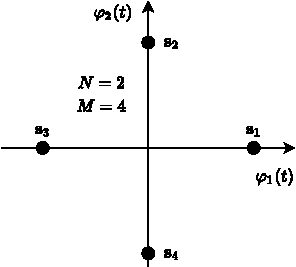
\includegraphics[width=0.98\linewidth]{Constellation1.pdf}
			\end{figure}
		\end{column}
	\end{columns}	
}

\subsection{Constelação de Sinais}
\pag{
	\frametitle{Constelação de Sinais}
	\begin{itemize}
		\item Para \textbf{esquemas lineares de modulação passa-faixa}, as funções de base que compõem o espaço de $N = 2$ dimensões são:
		\begin{block}{Funções Base (Modulações Lineares Passa-faixa)}
			\begin{subequations}
				\begin{align}
				        \varphi_{1}(t) = \sqrt{\frac{2}{E_{g}}}g(t)\cos(2\pi f_{c} t),   \\
				        \varphi_{2}(t) = -\sqrt{\frac{2}{E_{g}}}g(t)\sin(2\pi f_{c} t), \label{eq:MaxE}
				\end{align}
			\end{subequations}
		\end{block}
em que $g(t)$ é o pulso de formatação em banda base com energia $E_{g}$;
		\begin{block}{Condição de Ortogonalidade das Funções Base}
			\begin{equation}
				G(f)\star G(f)\vert_{f = \pm 2f_{c}} = 0,
			\end{equation}
		\end{block}
em que $G(f)$ é a transformada de Fourier do pulso $g(t)$.
	\end{itemize}
}

\subsection{Operações no Espaço de Sinais}
\pag{
	\frametitle{Operações no Espaço de Sinais}
	\begin{itemize}
		\item Para um conjunto de funções de base fixo, é valido afirmar que o \textbf{produto interno entre dois sinais reais} $s_{i}(t)$ e $s_{j}(t)$ é igual ao \textbf{produto interno vetorial} entre os vetores $\mathbf{s}_{i}$ e $\mathbf{s}_{j}$:
		\begin{block}{Produto Interno entre Sinais Reais}
			\begin{equation}
				\langle s_{i}(t), s_{j}(t)\rangle = \int_{0}^{T} s_{i}(t) s_{j}(t) dt = \langle \mathbf{s}_{i}, \mathbf{s}_{j}\rangle = \mathbf{s}_{i}^{T} \mathbf{s}_{j} = \sum_{m = 1}^{N} s_{im}s_{jm};
			\end{equation}
		\end{block}
		\begin{block}{Energia de um Sinal Real}
			\begin{equation}
				E_{s_{i}} = \int_{0}^{T}s_{i}^{2}(t)dt = \langle \mathbf{s}_{i}, \mathbf{s}_{i}\rangle =  \mathbf{s}_{i}^{T} \mathbf{s}_{i} = \sum_{m = 1}^{N} s_{im}^2 \triangleq \norm{\mathbf{s}_{i}}^2.
			\end{equation}
		\end{block}
	\end{itemize}
}

\section{Esquemas de Modulação}
\subsection{Constelação \textit{Pulse Amplitude Modulation} (PAM)}
\pag{
	\frametitle{Constelação \textit{Pulse Amplitude Modulation} (PAM)}
	\begin{itemize}
		\item	Na modulação M-PAM, a \textbf{informação é codificada na amplitude do sinal};
		\item 	O sinal M-PAM transmitido em um tempo de sinalização é dado por:
		\begin{block}{Sinal M-PAM}
			\begin{equation}
				s_{i}(t) = \Re\left\{\underbrace{A_{i}\sqrt{\frac{2}{E_{g}}}g(t)}_{\text{Equivalente banda base}}e^{j2\pi f_{c}t}\right\} = \underbrace{A_{i}\sqrt{\frac{2}{E_{g}}}g(t)\cos( 2\pi f_{c} t )}_{\text{Sinal passa-faixa}}, t \in [0,T],
			\end{equation}
			\vspace{-0.5cm}
				\begin{itemize}
					\item \textbf{Amplitude do Sinal Modulado}: $A_{i} = ( 2i - 1 - M)d$;
					\item \textbf{Dimensão do Espaço de Sinais}: $N = 1$;
					\item \textbf{Função Base}: $\varphi_{1}(t) = \sqrt{\frac{2}{E_{g}}}g(t)\cos( 2\pi f_{c} t )$.
				\end{itemize}
		\end{block}
	\end{itemize}
}

\pag{
	\frametitle{Constelação \textit{Pulse Amplitude Modulation} (PAM)}
	\begin{block}{Energia do Sinal M-PAM}
		\begin{equation}
			\begin{aligned}
				E_{s_{i}} &= \int_{0}^{T} A_{i}^{2}\frac{2}{E_{g}}g(t)^2 \cos^2( 2\pi f_{c} t ) dt \\
				&= A_{i}^{2}\frac{1}{E_{g}}\int_{0}^{T} g(t)^2 dt \cdots \\
				&+ A_{i}^{2}\frac{1}{E_{g}}\underbrace{\int_{0}^{T} g(t)^2\cos( 4\pi f_{c} t ) dt}_{\approx 0 \;(\text{Condição de Ortogonalidade})} \\
				&= A_{i}^2;
			\end{aligned}
		\end{equation}
	\end{block}
	\begin{block}{Energia Média dos Símbolos M-PAM (Símbolos Equiprováveis)}
		\begin{equation}
			\bar{E_{s}} = \frac{1}{M}\sum_{i = 1}^{M}E_{s_{i}} =  \frac{1}{M}\sum_{i = 1}^{M} A_{i}^2 = \frac{M^2 - 1}{3}d^2.
		\end{equation}
	\end{block}		
}

\pag{
	\frametitle{Constelação \textit{Pulse Amplitude Modulation} (PAM)}
	\begin{itemize}
		\item Sabendo que para uma constelação $M$-ária, cada símbolo representa uma sequência de $k = \log_{2}(M)$ bits, a \textbf{energia média necessária para transmitir um símbolo binário} é:
	\begin{block}{Energia Média por Bit (M-PAM)}
		\begin{equation}
			\bar{E_{b}} = \frac{\bar{E_{s}}}{\log_{2}(M)} = \frac{M^2 - 1}{3\log_{2}(M)}d^2.
		\end{equation}
	\end{block}
	\end{itemize}		
	\begin{figure}[!htb]
		\centering
		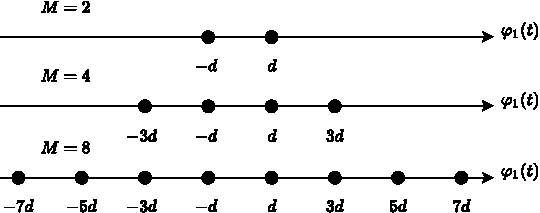
\includegraphics[width=0.8\linewidth]{PAM_C1.pdf}
	\end{figure}	
}

\pag{
	\frametitle{Constelação \textit{Pulse Amplitude Modulation} (PAM)}
	\begin{itemize}
		\item O mapeamento da constelação de símbolos em sequências binárias é geralmente feito por meio da \textbf{codificação Gray}, em que \textbf{sequências binárias associadas à símbolos adjacentes diferem em apenas um bit}.
	\end{itemize}
	\begin{figure}[!htb]
		\centering
		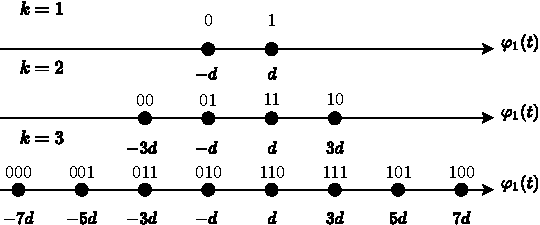
\includegraphics[width=0.9\linewidth]{PAM_C2.pdf}
	\end{figure}
}


\pag{
	\frametitle{Constelação \textit{Pulse Amplitude Modulation} (PAM)}
	\begin{figure}[!htb]
		\centering
		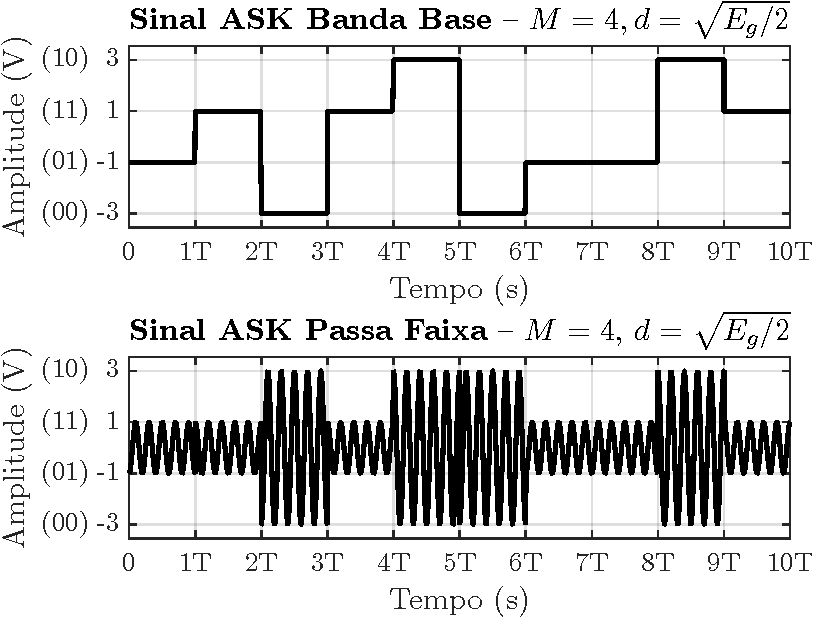
\includegraphics[width=0.9\linewidth]{SinalASK.pdf}
	\end{figure}	
}

\subsection{Constelação \textit{Quadrature Amplitude Modulation} (QAM)}

\pag{
	\frametitle{Constelação \textit{Quadrature Amplitude Modulation} (QAM)}
	\begin{itemize}
		\item Na modulação M-QAM, os \textbf{bits de informação são codificados na amplitude e na fase} do sinal transmitido (dois graus de liberdade);
		\begin{block}{Sinal M-QAM}
			\vspace{-0.5cm}
			\begin{equation}
				\begin{aligned}
				s_{i}(t) &= \Re\left\{\underbrace{(A_{i} + jB_{i})\sqrt{\frac{2}{E_{g}}}g(t)}_{\text{Equivalente banda base}}e^{j2\pi f_{c}t}\right\} \\
				&= A_{i}\sqrt{\frac{2}{E_{g}}}g(t)\cos( 2\pi f_{c} t ) - B_{i}\sqrt{\frac{2}{E_{g}}}g(t)\sin( 2\pi f_{c} t ), t \in [0,T],
				\end{aligned}
			\end{equation}
			\vspace{-0.5cm}
				\begin{itemize}
					\item \textbf{Amplitude do Sinal Modulado}: $A_{i}, B_{i} \in \{( 2i - 1 - \sqrt{M})d\}_{i = 1}^{\sqrt{M}}$;
					\item \textbf{Dimensão do Espaço de Sinais}: $N = 2$;
					\item \textbf{Função Base}: $\varphi_{1}(t) = \sqrt{\frac{2}{E_{g}}}g(t)\cos( 2\pi f_{c} t )$, $\varphi_{2}(t) = -\sqrt{\frac{2}{E_{g}}}g(t)\sin( 2\pi f_{c} t )$.
				\end{itemize}
		\end{block}
	\end{itemize}
}


\pag{
	\frametitle{Constelação \textit{Quadrature Amplitude Modulation} (QAM)}
	\begin{itemize}
		\item Alternativamente, os sinais M-QAM podem ser escritos na seguinte forma:
		\begin{block}{Sinal M-QAM}
			\begin{equation}
				\begin{aligned}
				s_{i}(t) &= \Re\left\{\underbrace{(V_{i}e^{j\phi_{i}})\sqrt{\frac{2}{E_{g}}}g(t)}_{\text{Equivalente banda base}}e^{j2\pi f_{c}t}\right\} \\
				&= V_{i}\sqrt{\frac{2}{E_{g}}}g(t)\cos( 2\pi f_{c} t + \phi_{i} ), t \in [0,T],
				\end{aligned}
			\end{equation}
			\vspace{-0.5cm}
				\begin{itemize}
					\item \textbf{Amplitude do Sinal Modulado}: $V_{i} = \sqrt{(A_{i}^2 + B_{i}^2)}$;
					\item \textbf{Fase do Sinal Modulado}: $\phi_{i} = \tan^{-1}(B_{i} / A_{i})$.
				\end{itemize}
		\end{block}
	\end{itemize}	
}

\pag{
	\frametitle{Modulador QAM}
			\begin{figure}[!h]
				\centering
			  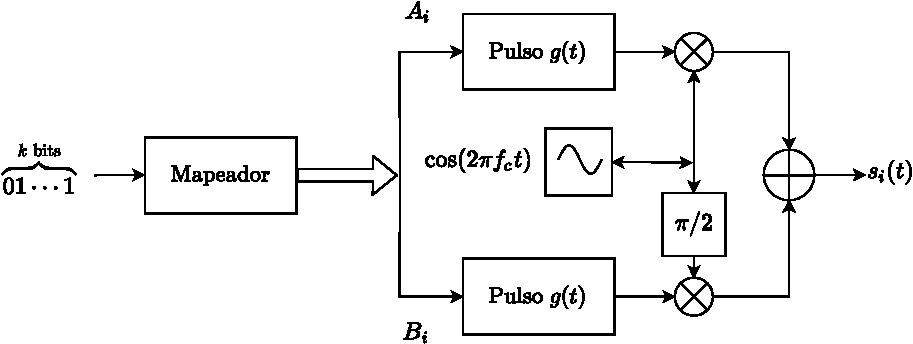
\includegraphics[width = 0.95\linewidth]{QAMMod.pdf}
				\label{QAMMod}
			\end{figure}
}


\pag{
	\frametitle{Constelação \textit{Quadrature Amplitude Modulation} (QAM)}
	\begin{block}{Energia do Sinal M-QAM}
		\begin{equation}
			\begin{aligned}
				E_{s_{i}} &= \int_{0}^{T} s_{i}(t)^{2}dt = \norm{\mathbf{s}_{i}}^2 = A_{i}^2 + B_{i}^2 = V_{i}^2;
			\end{aligned}
		\end{equation}
	\end{block}
	\begin{block}{Energia Média dos Símbolos M-QAM (Símbolos Equiprováveis)}
		\begin{equation}
			\bar{E_{s}} = \frac{1}{M}\sum_{i = 1}^{M}E_{s_{i}} = \frac{4}{M}\sum_{n = 1}^{\sqrt{M}/2}\sum_{m = 1}^{\sqrt{M}/2}(2n - 1 )^2 d^2 + (2j-1)^2d^2 = \frac{2}{3}(M - 1)d^2;
		\end{equation}
	\end{block}
		\begin{block}{Energia Média por Bit (M-QAM)}
		\begin{equation}
			\bar{E_{b}} = \frac{2(M - 1)d^2}{3\log_{2}(M)}.
		\end{equation}
		\end{block}
}

\pag{
	\frametitle{Constelação \textit{Quadrature Amplitude Modulation} (QAM)}
			\begin{figure}[!h]
				\centering
			  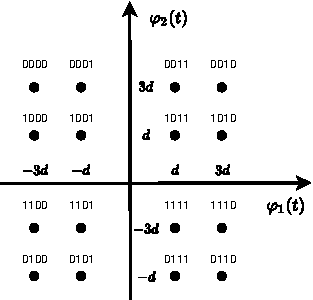
\includegraphics[width = 0.65\linewidth]{QAM_C1.pdf}
				\label{QAMMod}
			\end{figure}
}

\pag{
	\frametitle{Exemplo de Sinal QAM ($k = 4$~\textit{bits}, $M = 16$)}
			\begin{figure}[!h]
				\centering
			  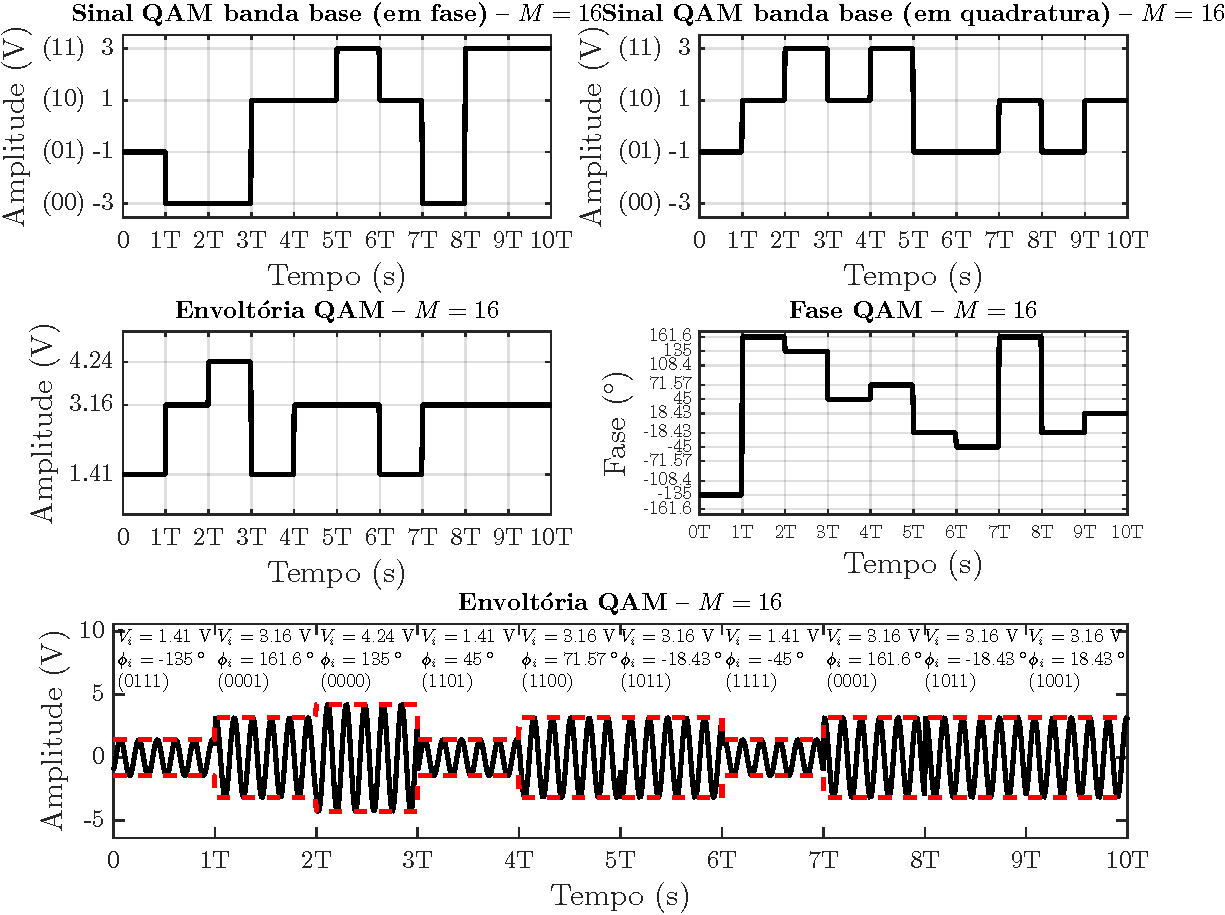
\includegraphics[width = 0.85\linewidth]{SinalQAM.pdf}
				\label{SinalQAM}
			\end{figure}
}

\pag{
	\begin{center}
		\resizebox{0.7\textwidth}{!}{%
  		\animategraphics[autoplay,loop]{1}{ConstVariation}{}{}
		}
	\end{center}
}

\subsection{Densidade Espectral de Potência dos Sinais Modulados}
\pag{
	\frametitle{Densidade Espectral de Potência dos Sinais Modulados}
	\begin{itemize}
		\item A partir da densidade espectral de potência (DEP), é possível determinar a \textbf{largura de faixa} requerida para a transmissão do sinal modulado;
		\item Para o cálculo da DEP, a sequência de informação é modelada por uma \textbf{sequência de variáveis aleatórias discretas};
		\item O sinal modulado passa-faixa pode ser modelado como um processo estocástico descrito por $v(t) = \Re\{\tilde{v}(t)e^{j2\pi f_c t}\}$, em que $\tilde{v}(t)$ é o \textbf{equivalente em banda base};
		\begin{block}{Sinal em Banda Básica}
			\vspace{-0.15cm}
			\begin{equation}
				\tilde{v}(t) = \sum_{k = -\infty}^{\infty}\alpha_{k}g( t - kT );
			\end{equation}
			\vspace{-0.5cm}
			\begin{itemize}
				\item \textbf{Índice do tempo}: $k$;
				\item \textbf{Sequência de variáveis aleatórias discretas}: $\alpha_{k} \in \mathbb{C}$;
				\item \textbf{Pulso de formatação}: $g(t)$.
			\end{itemize}
		\end{block}
	\end{itemize}
}

\pag{
	\frametitle{Densidade Espectral de Potência dos Sinais Modulados}
	\begin{itemize}
		\item Pode-se assumir que o processo estocástico discreto $\alpha_{k}$ é \textbf{estacionário em sentido amplo} (ESA);
		\item Se $\alpha_{k}$ é ESA, pode-se demonstrar que o processo $\tilde{v}(t)$ é \textbf{ciclo-estacionário no sentido amplo} (CESA) com período $T$;
	\begin{block}{Média e Autocorrelação de $\alpha_{k}$}
		\vspace{-0.5cm}
			\begin{subequations}
				\begin{align}
				        \mathbf{E}\{\alpha_{k}\} &= \eta_{\alpha},   \\
				        \mathbf{E}\{\alpha_{k}^{*}\alpha_{k+n}\} &= r_{\alpha}[n], \label{eq:MaxE}
				\end{align}
			\end{subequations}
	\end{block}	
	\begin{block}{Densidade Espectral de Potência do Processo $\tilde{v}(t)$ CESA}
		\begin{equation}
			S_{\tilde{v}}(f) = \frac{1}{T}\abs{G(f)}^2R_{\alpha}(f),
		\end{equation}
		\vspace{-0.3cm}
		\begin{itemize}
			\item \textbf{Transformada de Fourier do pulso de formatação}: $G(f)$;
			\item \textbf{Transformada de Fourier do tempo discreto de $r_{\alpha}[n]$}: $R(f)$.
		\end{itemize}
	\end{block}		
	\end{itemize}		
}

\pag{
	\frametitle{Densidade Espectral de Potência dos Sinais Modulados}
	\begin{itemize}
		\item Os esquemas de modulações lineares equiprováveis com constelações simétricas em torno da origem, \textit{e.g.}, M-PAM (M-ASK) e M-QAM têm \textbf{símbolos de informação com média nula} ($\eta_{\alpha} = 0$);
		\item A DEP do sinal em banda básica $\tilde{v}(t)$ depende do pulso de formatação $g(t)$ e da autocorrelação entre os símbolos da sequência de informação;
		\item Considerando que as sequências são descorrelacionadas, a DEP é descrita por:
	\begin{block}{DEP do Processo CESA $\tilde{v}(t)$ com Sequências Descorrelacionadas de Média Nula}
		\begin{equation}
			S_{\tilde{v}}(f) = \frac{\sigma_{\alpha}^2}{T}|G(f)|^2,
		\end{equation}
	\end{block}
em que $\sigma_{\alpha}^{2}$ é a potência da sequência $\alpha_{k}$.
	\end{itemize}
}


\pag{
	\frametitle{Densidade Espectral de Potência dos Sinais Modulados}
	\begin{block}{DEP do Sinal QAM (Pulso Retangular)}
		\begin{equation}
			S_{\tilde{v}}(f) = T\sigma_{\alpha}^2\mathrm{sa}(\pi f T)^2.
		\end{equation}
	\end{block}
	\begin{figure}[!h]
		\centering
	  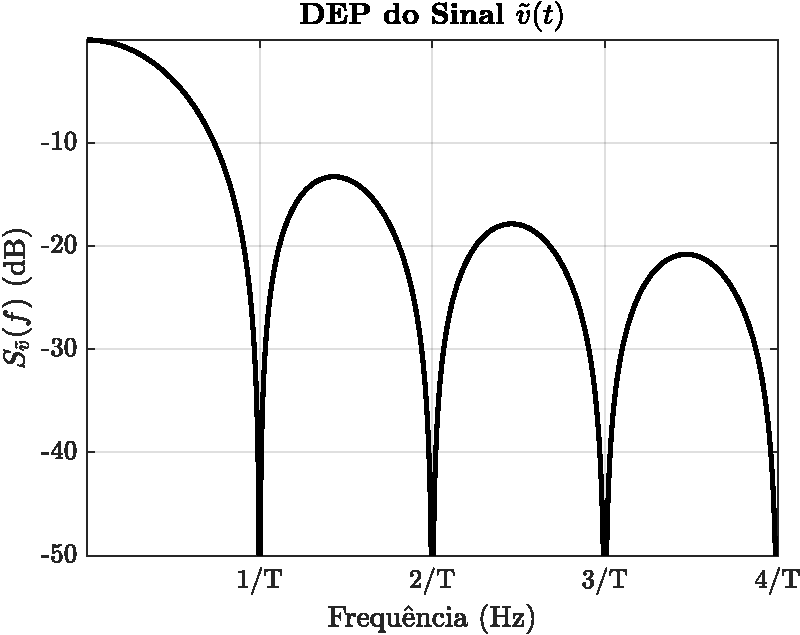
\includegraphics[width = 0.6\linewidth]{QAMDEP.pdf}
		\label{SinalQAM}
	\end{figure}
}

%\begin{frame}
%\frametitle{}
%\begin{center}
%  {\Huge Obrigado!\\}
%  {\Huge Contato:\\} 
%  {\huge higo.silva@ee.ufcg.edu.br\\} 
%\end{center}
%\end{frame}

\end{document}
